\mode*

\section{Inbyggda funktioner}

\begin{frame}
  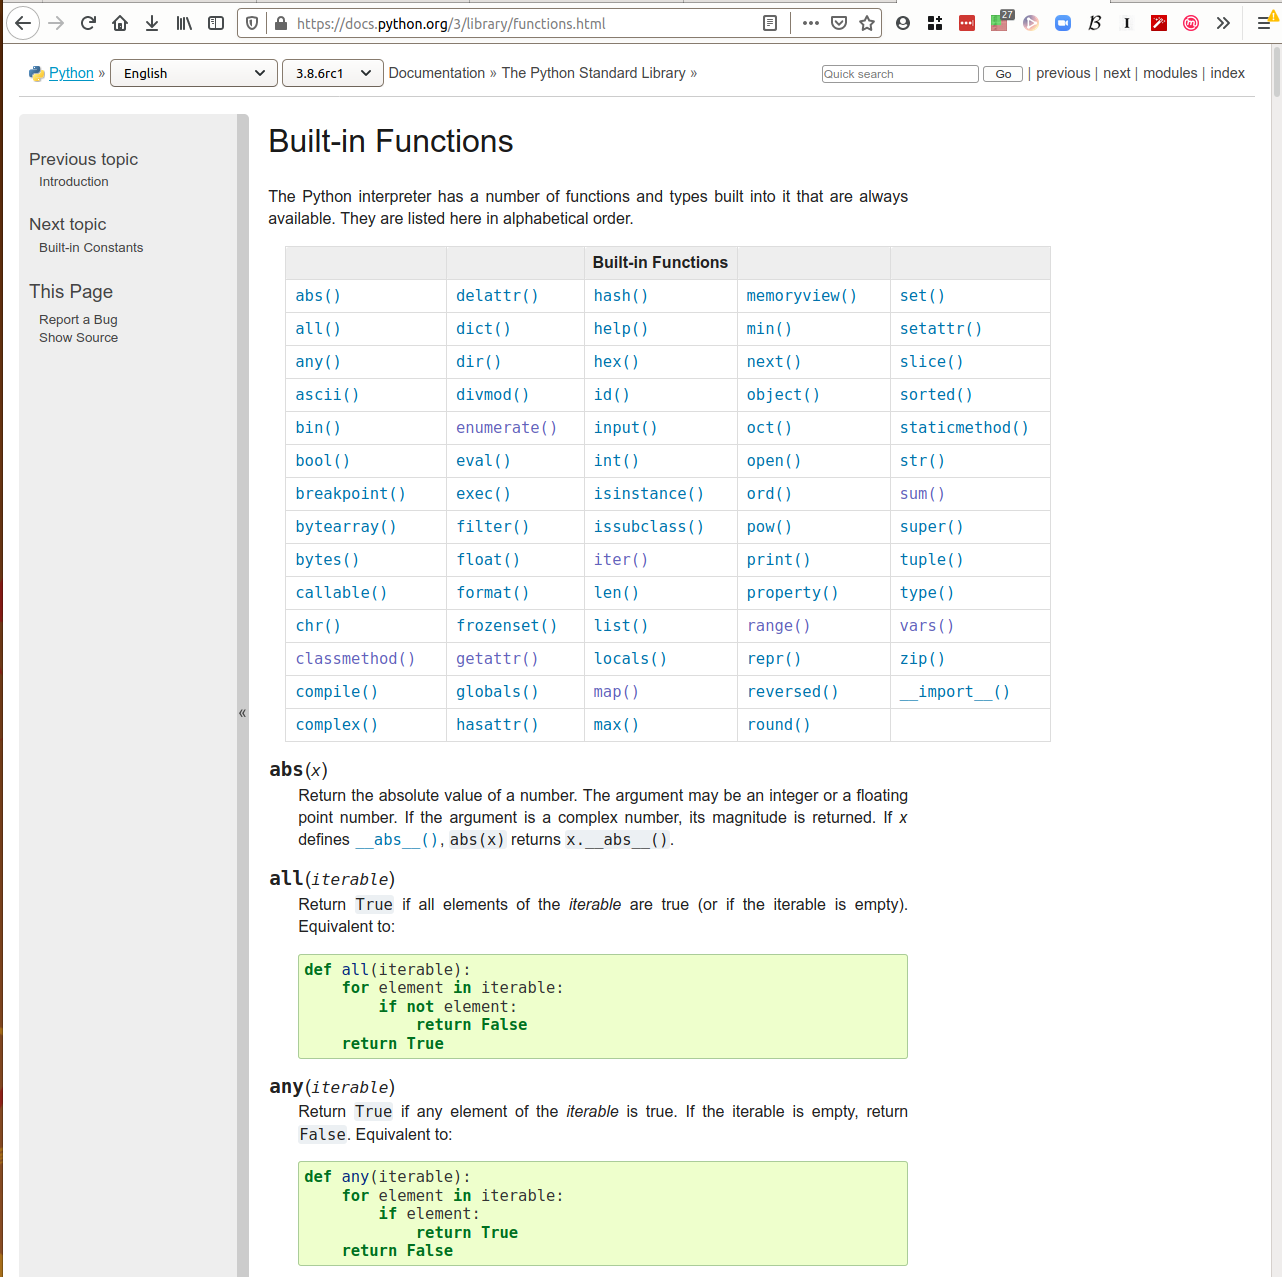
\includegraphics[width=\columnwidth]{figs/docs-built-in.png}
\end{frame}

\subsection{map() och filter()}

\begin{frame}[fragile]
  \begin{example}[mapping.py, del 1]
    \inputminted[firstline=3,lastline=15]{python}{examples/mapping.py}
  \end{example}
\end{frame}

\begin{frame}[fragile]
  \begin{example}[mapping.py, del 2]
    \inputminted[firstline=16]{python}{examples/mapping.py}
  \end{example}
\end{frame}

\begin{frame}[fragile]
  \begin{example}[filtering.py, del 1]
    \inputminted[firstline=3,lastline=15]{python}{examples/filtering.py}
  \end{example}
\end{frame}

\begin{frame}[fragile]
  \begin{example}[filtering.py, del 2]
    \inputminted[firstline=21]{python}{examples/filtering.py}
  \end{example}
\end{frame}

\subsection{Namnlösa (lambda-)funktioner}

\begin{frame}[fragile]
  \begin{example}[filter-lambda.py]
    \inputminted{python}{examples/filter-lambda.py}
  \end{example}
\end{frame}

\begin{frame}[fragile]
  \begin{example}[any-all.py, del 1]
    \inputminted[firstline=7,lastline=18]{python}{examples/any-all.py}
  \end{example}
\end{frame}

\begin{frame}[fragile]
  \begin{example}[any-all.py, del 2]
    \inputminted[firstline=20]{python}{examples/any-all.py}
  \end{example}
\end{frame}

\subsection{zip() och enumerate()}

\begin{frame}[fragile]
  \begin{example}[enum.py]
    \inputminted{python}{examples/enum.py}
  \end{example}
\end{frame}

\begin{frame}[fragile]
  \begin{example}[zip.py]
    \inputminted{python}{examples/zip.py}
  \end{example}
\end{frame}

